\documentclass{beamer}
\usepackage[utf8x]{inputenc}
\usepackage[czech]{babel}
\usepackage{booktabs}
\usepackage{listings}

\usetheme[pageofpages=of,% String used between the current page and the
                         % total page count.
          bullet=circle,% Use circles instead of squares for bullets.
          titleline=true,% Show a line below the frame title.
	  titlepagelogo=opensuse,
          alternativetitlepage=true,% Use the fancy title page.
          ]{Torino}

\setbeamerfont{title}{series=\bfseries,size=\LARGE}
\author{Tom\'{a}\v{s} Chv\'{a}tal\newline {\small openSUSE Team}}
\title{Autotools workshop}
\date{2013/07/19}

\AtBeginSection[]
{
	\setbeamercolor{background canvas}{bg=chameleongreen3}
	\begin{frame}[plain]
		\begin{center}\begin{huge}\textcolor{white}{\secname}\end{huge}\end{center}
	\end{frame}
	\setbeamercolor{background canvas}{bg=}
}

\AtBeginSubsection[]
{
	\setbeamercolor{background canvas}{bg=chameleongreen3}
	\begin{frame}[plain]
		\begin{center}\begin{huge}\textcolor{white}{\subsecname}\end{huge}\end{center}
	\end{frame}
	\setbeamercolor{background canvas}{bg=}
}

\begin{document}

\begin{frame}[t,plain]
\titlepage
\end{frame}

\section{Introduction}

\begin{frame}[t]{Who the hell is Tomáš Chvátal}
	\begin{itemize}
	\item SUSE Employee since 2011 (QA, openSUSE)
	\item Packager of Libreoffice and various other stuff for openSUSE
	\item openSUSE promoter and volunteer
	\item Gentoo developer since fall 2008 and Council member since 2010
	\end{itemize}
	\begin{center}As this is workshop, remember to ask questions if in doubt or curious. I don't bite, really.\end{center}
\end{frame}

\section{Autotools process}

\begin{frame}{Complete autotools process}
	\begin{figure}
	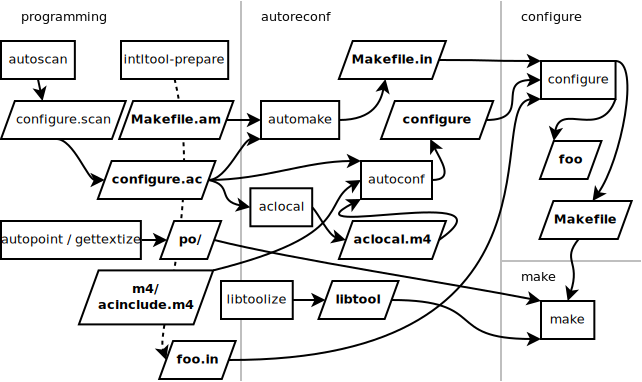
\includegraphics[width= 1.0\linewidth]{autotools.png}
	\end{figure}
\end{frame}

\begin{frame}{Simplified autotools process}
	\begin{figure}
	\includegraphics[width= 1.0\linewidth]{autotools_simple.png}
	\end{figure}
\end{frame}

\begin{frame}{How does deploying look}
	\begin{tabular}{|l|l|}
	\toprule
	Developer & Consumer \\
	\midrule
	\$ cd git-repo/ & \$ wget "uploaded tarball" \\
	\$ sh autogen.sh & \$ unpack "uploaded tarball" \\
	\$ ./configure & \$ ./configure --enable-this --disable-that \\
	\$ make distcheck & \$ make -jVALUE \\
	"upload tarball" & \$ make install \\
	\bottomrule
	\end{tabular}
\end{frame}

\section{Writting autotools for dummies}

\subsection{Autoconf aka configure.ac}

\begin{frame}[t]{What is autogen.sh}
	\begin{itemize}
	\item \url{http://tinyurl.com/q596zjt} \\
	\item Shorter version is just to run "autoreconf -vi"
	\end{itemize}
\end{frame}

\begin{frame}[t]{Defining version}
	\begin{small}
	\lstinputlisting{autoconfinit.txt}
	\end{small}
\end{frame}

\begin{frame}[t]{Finding used apps/libs}
	\begin{small}
	\lstinputlisting{autoconfappsdetection.txt}
	\end{small}
\end{frame}

\begin{frame}[t]{Hand-searching for libraries}
	\begin{small}
	\lstinputlisting{autoconfhandlib.txt}
	\end{small}
\end{frame}

\begin{frame}[t]{Automagicness in autoconf}
	\begin{small}
	\lstinputlisting{autoconfautomagicness.txt}
	\end{small}
\end{frame}

\begin{frame}[t]{Werror handling}
	\begin{small}
	\lstinputlisting{autoconfwerror.txt}
	\end{small}
\end{frame}

\begin{frame}[t]{Generate results}
	\begin{small}
	\lstinputlisting{autoconfresults.txt}
	\end{small}
\end{frame}

\begin{frame}[t]{m4 macros}
	\begin{small}
	\lstinputlisting{m4macros.txt}
	\end{small}
\end{frame}

\subsection{Automake aka Makefile.am}

\begin{frame}[t]{Non-recursive Makefiles}
	\begin{itemize}
	\item Easier to see the changes in one file in top \$(srcdir)
	\item Faster with paralelization, because of the depgraph calculations
	\item Easier to write the stack as you always start from the top
	\end{itemize}
\end{frame}

\begin{frame}[t]{Basic declarations}
	\begin{small}
	\lstinputlisting{automakedefaultvars.txt}
	\end{small}
\end{frame}

\begin{frame}[t]{Adding sources}
	\begin{small}
	\lstinputlisting{automakesources.txt}
	\end{small}
\end{frame}

\begin{frame}[t]{Adding headers}
	\begin{small}
	\lstinputlisting{automakeinclude.txt}
	\end{small}
\end{frame}

\begin{frame}[t]{Creating tests}
	\begin{small}
	\lstinputlisting{automaketests.txt}
	\end{small}
\end{frame}

\begin{frame}[t]{Creating custom rules}
	\begin{small}
	\lstinputlisting{automakecustomrules.txt}
	\end{small}
\end{frame}

\subsection{Libtool}

\begin{frame}{Libtool versioning}
	\begin{itemize}
	\item Start with version information of ‘0:0:0’ for each libtool library
	\item Update the version information only immediately before a public release of your software. More frequent updates are unnecessary, and only guarantee that the current interface number gets larger faster
	\item If the library source code has changed at all since the last update, then increment revision (‘c:r:a’ becomes ‘c:r+1:a’)
	\item If any interfaces have been added, removed, or changed since the last update, increment current, and set revision to 0
	\item If any interfaces have been added since the last public release, then increment age
	\item If any interfaces have been removed or changed since the last public release, then set age to 0
	\end{itemize}
\end{frame}

\begin{frame}[t]{configure.ac changes}
	\begin{small}
	\lstinputlisting{autoconflibtool.txt}
	\end{small}
\end{frame}

\begin{frame}[t]{Makefile.am changes}
	\begin{small}
	\lstinputlisting{automakelibtool.txt}
	\end{small}
\end{frame}

\section{Lets try to write a buildsystem}

\begin{frame}{Lets write a buildsystem for sax3}
\url{https://github.com/openSUSE/sax3/tree/kill-ui-library}
\end{frame}

\section{Reading}

\begin{frame}{Reading}
	\begin{figure}
	\includegraphics[width= 0.4\linewidth]{mythbuster.png}
	\end{figure}
\end{frame}

\section{Endnote}

\begin{frame}{Suse is hiring}
	\begin{figure}
	\includegraphics[width= 0.8\linewidth]{suse_hiring.png}
	\end{figure}
\end{frame}

\begin{frame}{Thanks}
	\begin{center}
	Thank you for your attention.
	\end{center}
\end{frame}

\end{document}

